%%%%%%%%%%%%%%%%%%%%%%%%%%%%%%%%%%%%%%%%%%%%%%%%%%%%%%%%%%%%%%%%%%%%%%%%%%%%%%%%%%
\begin{frame}[fragile]\frametitle{}
\begin{center}
{\Large Different Large Language Models}

\end{center}
\end{frame}

%%%%%%%%%%%%%%%%%%%%%%%%%%%%%%%%%%%%%%%%%%%%%%%%%%%%%%%%%%%
\begin{frame}[fragile]\frametitle{Transformer Models}



		\begin{center}
		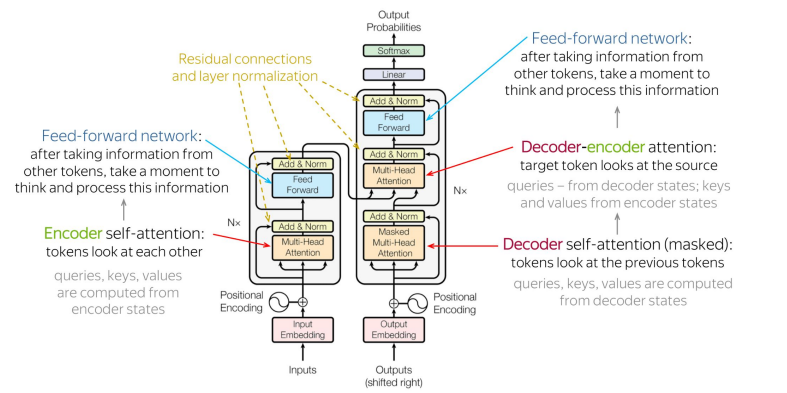
\includegraphics[width=\linewidth,keepaspectratio]{promptengg81}

		{\tiny (Ref: The Complete Prompt Engineering for AI Bootcamp (2023))}
		\end{center}	

\end{frame}



%%%%%%%%%%%%%%%%%%%%%%%%%%%%%%%%%%%%%%%%%%%%%%%%%%%%%%%%%%%
\begin{frame}[fragile]\frametitle{GPT3}


\begin{columns}
    \begin{column}[T]{0.6\linewidth}
		\begin{center}
		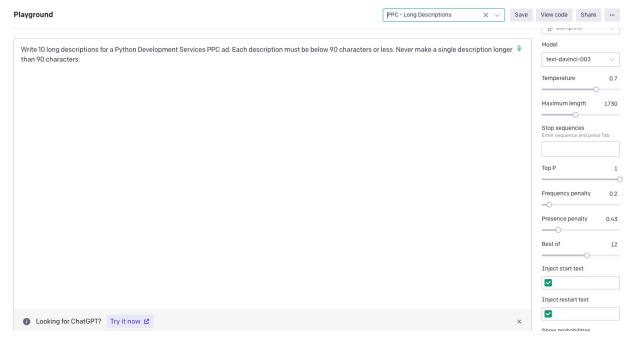
\includegraphics[width=\linewidth,keepaspectratio]{promptengg82}

		{\tiny (Ref: The Complete Prompt Engineering for AI Bootcamp (2023))}
		\end{center}	
    \end{column}
    \begin{column}[T]{0.4\linewidth}
		Created by OpenAI
		Access it with code or without (Playground https://platform.openai.com/playground)
    \end{column}
  \end{columns}
\end{frame}

%%%%%%%%%%%%%%%%%%%%%%%%%%%%%%%%%%%%%%%%%%%%%%%%%%%%%%%%%%%
\begin{frame}[fragile]\frametitle{GPT3 Features}


		\begin{center}
		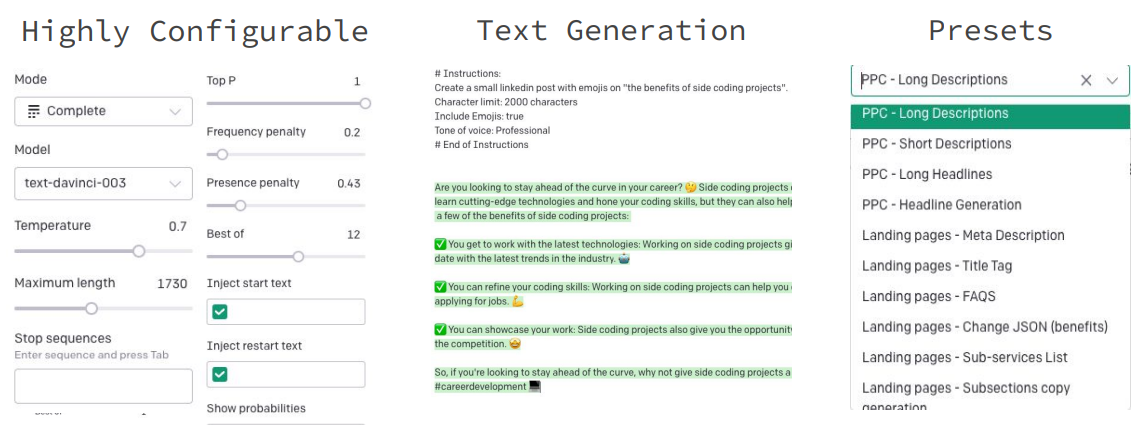
\includegraphics[width=\linewidth,keepaspectratio]{promptengg83}

		{\tiny (Ref: The Complete Prompt Engineering for AI Bootcamp (2023))}
		\end{center}	

\end{frame}


%%%%%%%%%%%%%%%%%%%%%%%%%%%%%%%%%%%%%%%%%%%%%%%%%%%%%%%%%%%
\begin{frame}[fragile]\frametitle{GPT3 Usecases}


		\begin{center}
		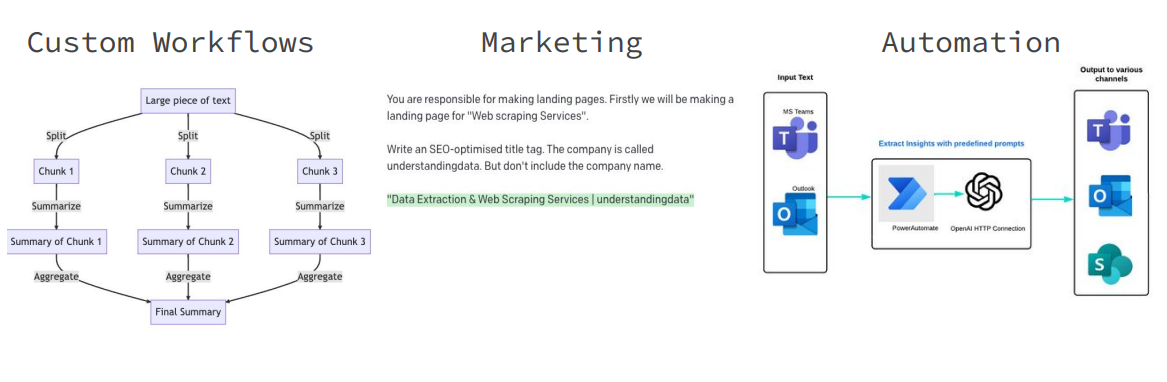
\includegraphics[width=\linewidth,keepaspectratio]{promptengg84}

		{\tiny (Ref: The Complete Prompt Engineering for AI Bootcamp (2023))}
		\end{center}	

\end{frame}

%%%%%%%%%%%%%%%%%%%%%%%%%%%%%%%%%%%%%%%%%%%%%%%%%%%%%%%%%%%
\begin{frame}[fragile]\frametitle{GPT3 Limitations}




\begin{itemize}
\item  Unlike ChatGPT, GPT-3 doesn’t store chat history, which can lead to you needing to re-inject the extra context into the
original prompt.
\item Tokens are currently limited to 4000 tokens per output. This includes both your initial prompt the text generated
from ChatGPT.

\end{itemize}	 

{\tiny (Ref: The Complete Prompt Engineering for AI Bootcamp (2023))}

\end{frame}


%%%%%%%%%%%%%%%%%%%%%%%%%%%%%%%%%%%%%%%%%%%%%%%%%%%%%%%%%%%
\begin{frame}[fragile]\frametitle{Bard}


\begin{columns}
    \begin{column}[T]{0.6\linewidth}
		\begin{center}
		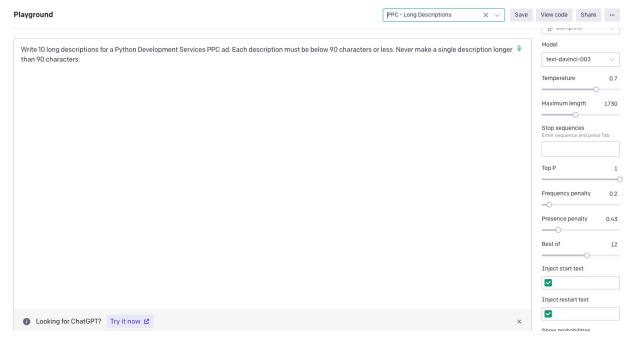
\includegraphics[width=\linewidth,keepaspectratio]{promptengg82}

		{\tiny (Ref: The Complete Prompt Engineering for AI Bootcamp (2023))}
		\end{center}	
    \end{column}
    \begin{column}[T]{0.4\linewidth}
		Created by Google
		Access it via chat https://bard.google.com/ or encounter it in search results
    \end{column}
  \end{columns}
\end{frame}